\documentclass[t]{beamer}
\usetheme[deutsch]{KIT}
\setbeamercovered{transparent}
\setbeamertemplate{navigation symbols}{}

\KITfoot{}
\usepackage[utf8]{inputenc}
\usepackage{ngerman}
\usenavigationsymbols

\title{OQAT - Objective Quality Assessment Toolkit}
\subtitle{PSE - Abschlusspräsentation im SS2012 den 00 September \\[0.3cm]
Alexander Monev $\cdot$ Artur Eckhart $\cdot$ Georg Ermantraut\\ $\cdot$ Johannes Sailer  $\cdot$ Sebastian
Leidig \\[0.3cm] Betreuer: Dipl.-Inform. Sebastian Kobbe}

\institute[ITEC]{Institut für Technische Informatik $\cdot$ Lehrstuhl für Eingebettete Systeme $\cdot$ Prof. Dr. Jörg Henkel	}
\TitleImage[height=\titleimageht]{img/oqatLogo}

\AtBeginSection[]
{
  \begin{frame}
    \frametitle{Übersicht}
    \tableofcontents[currentsection]
  \end{frame}
}

\begin{document}

\begin{frame}
	\maketitle
\end{frame}

\begin{frame}
	\frametitle{Übersicht}
	\addcontentsline{toc}{section}{}
	\tableofcontents
\end{frame}

\section{Aufgabenstellung}

\begin{frame}
	\frametitle{Aufgabenstellung}
	
		
			\begin{itemize}
				\item <+-> Videoencoder testen
				\item <+-> Videos verändern
				\item <+-> Videos analysieren
				% \item <+-> Wozu?
			\end{itemize}
			\begin{figure}
				\includegraphics<4->[scale=.32]{img/aufgabe.png}
			\end{figure}
		
				

\end{frame}
\begin{frame}
	\frametitle{Aufgabenstellung}
	\begin{center}
		\vspace*{\fill}
		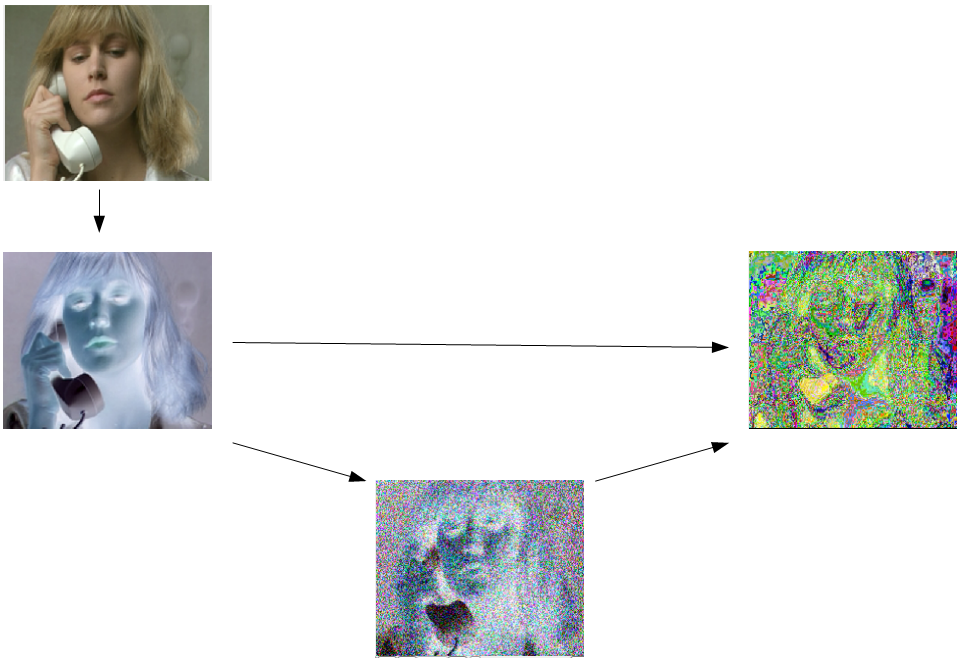
\includegraphics[scale=.35]{img/aufgabe2.png}
		\vspace*{\fill} ~\\
	\end{center}
\end{frame}


\section{Vorführung}


\section{Architektur}
\begin{frame}
\frametitle{Architekturmuster  MVVM}
\begin{minipage}{5,5cm}
\begin{center}
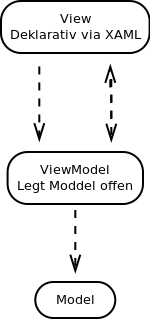
\includegraphics[scale=.5]{img/arch/mvvm.png}
\end{center}
\end{minipage}
\begin{minipage}{5,5cm}
\begin{itemize}
\itemsep1em
\item <+-> Model View ViewModel Architekturmuster
\item <+-> View deklarativ definiert
\item <+-> Databinding
\item <+-> Erweiterbarkeit durch Plugins
\item <+-> Verbesserte Testbarkeit
\end{itemize}
\end{minipage}
\end{frame}
\begin{frame}
\frametitle{Plugins}
\begin{center}
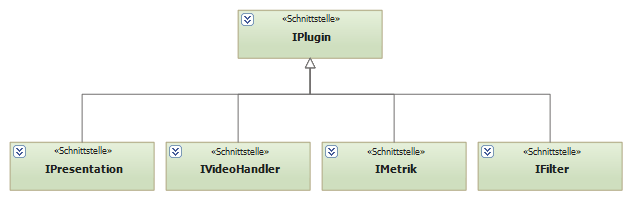
\includegraphics[scale=.5]{img/arch/IPluginStructure.png}
\end{center}
\begin{itemize}
\itemsep1em
\item <+-> Managed Extensibility Framework (MEF)
\item <+-> Kein Neustart notwendig
 \item <+-> Pluginmanager
\end{itemize}
\end{frame}
\begin{frame}
\frametitle{Von der View zum ViewModel}
\begin{center}
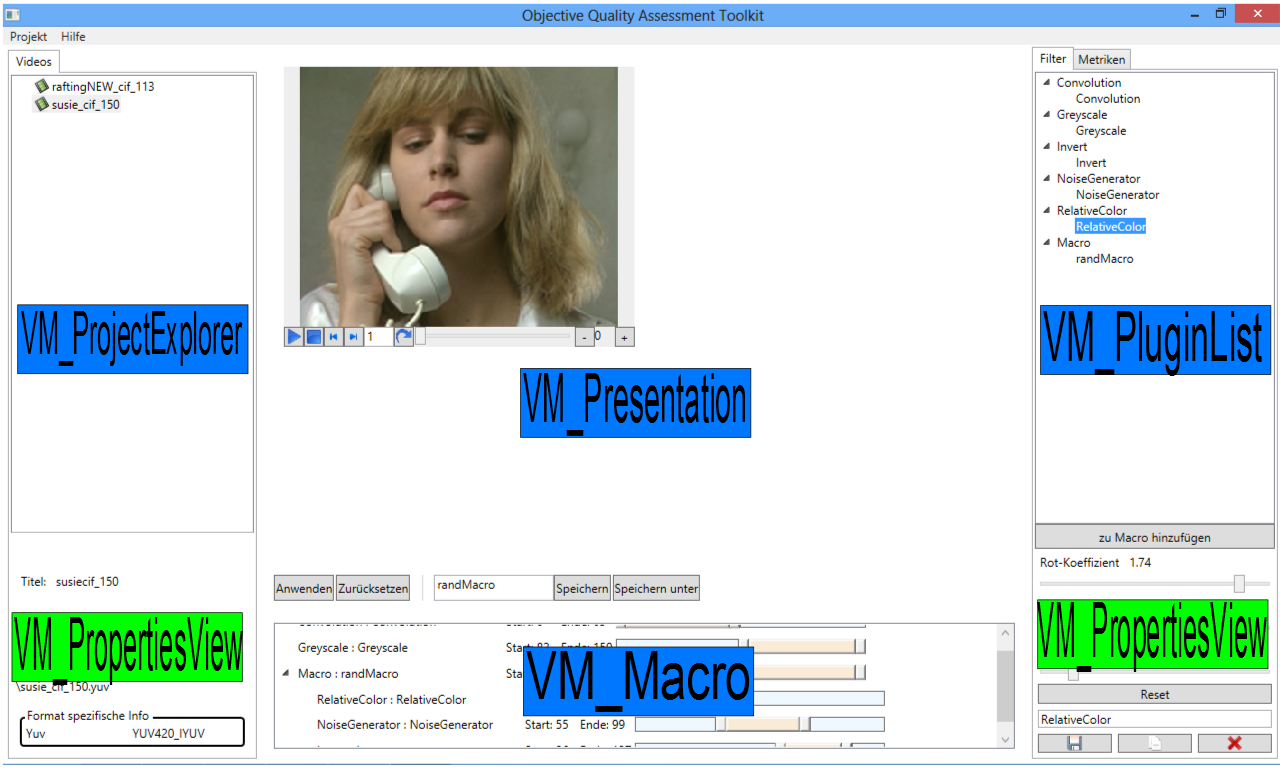
\includegraphics[scale=.23]{img/arch/generalOverview.png}
\end{center}
\end{frame}

\section{Entwicklungsumgebung}
\begin{frame}
	\frametitle{Entwicklungsumgebung}
	\begin{minipage}{5,5cm}
	\centering
	\raisebox{-2.5cm}[0pt]{
\includegraphics[scale=.2]{img/logos/csharp-logo.png}}
	\end{minipage}
	\begin{minipage}{5,5cm}
	\centering
	\raisebox{-2.5cm}[0pt]{
\includegraphics[scale=.4]{img/logos/visual-studio-2010-logo.png}}
	\end{minipage}
	\begin{minipage}{5,5cm}
	\centering
	\raisebox{-1.5cm}[0pt]{
\includegraphics[scale=.4]{img/libsFrameworks/git.png}}
	\end{minipage}
	\begin{minipage}{5,5cm}
	\centering
	\raisebox{-1.5cm}[0pt]{
\includegraphics[scale=1]{img/logos/texmaker-logo.png}}
	\end{minipage}
	\begin{minipage}{5,5cm}
	\centering
	\raisebox{-1.5cm}[0pt]{
\includegraphics[scale=.5]{img/logos/MEF-logo.jpg}}
	\end{minipage}
	\begin{minipage}{5,5cm}
	\centering
	\raisebox{-1.5cm}[0pt]{
\includegraphics[scale=.5]{img/libsFrameworks/aforgenetf.jpg}}
	\end{minipage}
\end{frame}
\section{Statistiken}
\begin{frame}
	\frametitle{Git Code Frequency}
	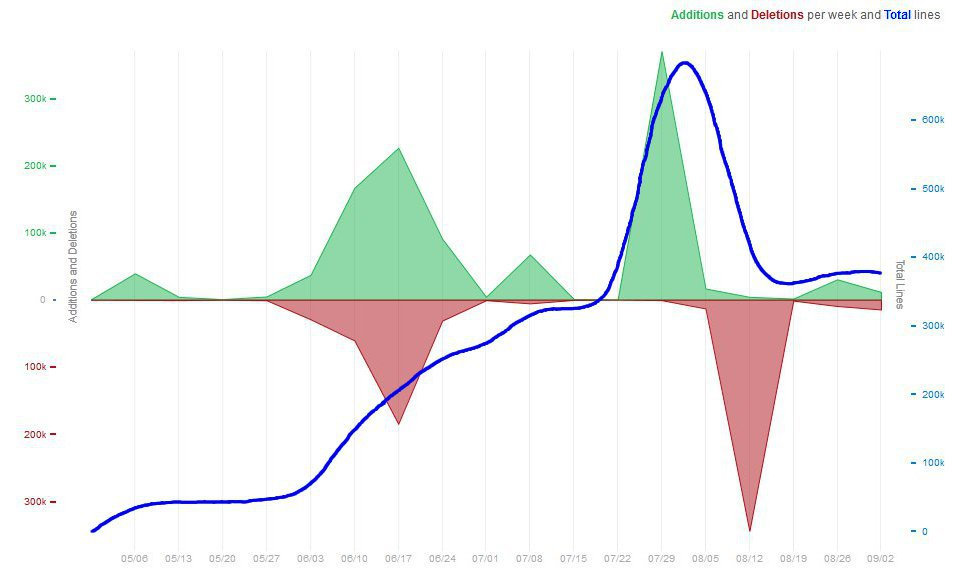
\includegraphics[scale=.33]{img/GitCodeFrequency.jpg}
	%\hyperlink{Git Code Frequency}{https://github.com/PSE-2012/MMWTV/graphs/code-frequency}
\end{frame}
\begin{frame}[c]
	\frametitle{Fakten}
	\begin{itemize}
		\item <+-> \begin{math}\sim\end{math} 26.000 Zeilen Code \raisebox{-1.5cm}[0pt]{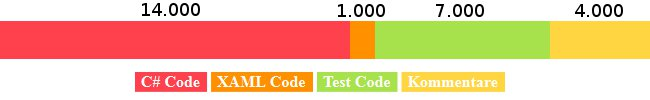
\includegraphics[scale=.5]{img/BarDiagramm-Zeilen.jpg}} %, C\# Code + XAML + Test + Kommentare
		%14.000 Zeilen C# Code
		%1.000 Zeilen XAML
		%7.000 Zeilen Test
		%4.000 Zeilen Kommentare
			\item <+-> 85 Klassen, 11 Interfaces
			%85 Klassen
			%53 Klassen Test
			%11 Interfaces
		\item <+-> Unittests: 82\% Codeabdeckung %Rest UI-Tests
		\item <+-> Wartbarkeit
		\includegraphics<4->[scale=.05]{img/DaumenHoch.jpg}
		\item <+-> 118 Issues, 843 Commits 
		\end{itemize}
		
	
\end{frame}


\section{Fazit}
\begin{frame}[c]
	\frametitle{Fazit}
	\framesubtitle{Was haben wir gelernt?}
	\begin{itemize}
	\itemsep1em
	\item <+-> Entwurf simpler gestalten
	\item <+-> Einarbeitungszeit
	\item <+-> Teamarbeit
	\item <+-> Schätzung von Zeitaufwand
	\end{itemize}
\end{frame}
\begin{frame}[c]
	\begin{center}
	Vielen Dank für Ihre Aufmerksamkeit.
	\end{center}
\end{frame}
\end{document} 
